%\tikzset
%{
%	treenode/.style = {circle, draw=black!60, fill=white!40, very thick, minimum size=6mm}
%}

\begin{figure}[H]
	\center

	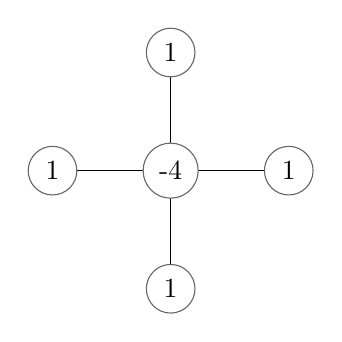
\begin{tikzpicture}%[level/.style={sibling distance = 2cm/#1, level distance = 3cm}]
	
	\def \xone{0};
	\def \yone{0};
	\def \h{1.5}	

	\coordinate (M) at (\xone ,\yone);
	\coordinate (L) at (\xone-\h ,\yone);
	\coordinate (R) at (\xone+\h ,\yone);
	\coordinate (O) at (\xone ,\yone+\h);
	\coordinate (U) at (\xone ,\yone-\h);
	\draw (L) -- (R);
	\draw (U) -- (O);

	%draw nodes
	\node[circle,draw=black!60, fill=white!40] at (M) {-4};
	\node[circle,draw=black!60, fill=white!40] at (L) {1};
	\node[circle,draw=black!60, fill=white!40] at (R) {1};
	\node[circle,draw=black!60, fill=white!40] at (O) {1};
	\node[circle,draw=black!60, fill=white!40] at (U) {1};

		
	\end{tikzpicture}
	
\caption{5-point stencil (second order accurate)}
\label{five_point}
\end{figure}
